\documentclass{resonance}
\usepackage[hidelinks]{hyperref}
\usepackage{xcolor}
\usepackage[cache=false]{minted}
\usemintedstyle{xcode}

\setlength{\fboxsep}{0pt}

\begin{document}

\title{Mathematical Simulations through Monte Carlo Methods}
\secondTitle{Fractal Trees and the Approximation of Pi}
\author{Akshansh Bhanjana - Aryan Gupta}

\maketitle
\authorIntro{\includegraphics[width=2cm]{akshansh}\\
Akshansh Bhanjana is a sophomore at Cluster Innovation Centre,
University of Delhi, currently majoring in Information Technology and Mathematical Innovations.\\
\authorIntro{\includegraphics[width=2cm]{aryan}\\
Aryan Gupta is a student at Cluster Innovation Centre,
University of Delhi, pursuing majors in Information Technology \& Mathematical Innovations.}}

\begin{abstract}
Algorithms involving Monte Carlo Methods are comparatively scalable. They see a lot of usage in physical systems. This method can reduce complex models to simpler events, which can be simulated with ease. This paper involves simulations of two such mathematical phenomena: Estimating the Value of Pi, and Fractal Trees.
\end{abstract}

\monthyear{June 2020}
\artNature{GENERAL ARTICLE}


\section*{Introduction}
In probability, we encounter various situations where an analytical solution cannot be calculated directly. This calculation may be difficult due to various reasons such as having many random variables, disturbances (noise) in the observations, etc.

The Monte Carlo Method came into existence around the 1940s by scientists involved in The Manhattan Project (which led to the development of the atomic bomb). Named after Monaco, a city infamous for its casinos and games of ‘chances’, its purpose was to use random input samples to understand a complex system. 

Nowadays, the Monte Carlo method provides usage in a wide range of risk analysis problems in almost every industry. These use-cases find prominence in professional fields such as finance, engineering, R\&D, and more.

\hspace{90pt}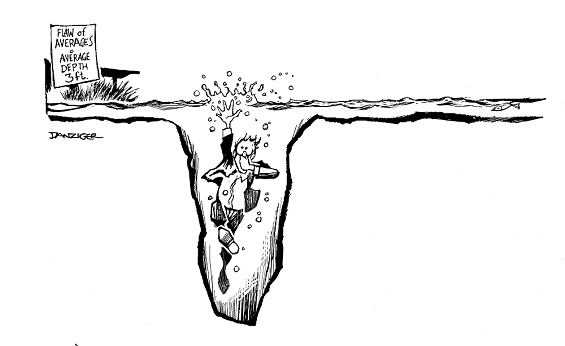
\includegraphics[width=3cm]{the-flaw-of-averages}

\scriptsize{\textbf{Figure 1}. The Flaw of Averages (Source: Sam L. Savage, Hoboken, NJ: John Wiley \& Sons, 2009)}

\pagebreak 

The Statistician, based on the (F)Law of Averages, believes that the river is safe to cross, with its average depth of 3 ft (0.91 m). In reality, the river is 6 inches deep around the banks, but 8 feet deep at the centre! The term 'average depth' therefore has no useful meaning. This Flaw of Averages, states that any plan based on average assumptions is wrong on average.
Similarily, taking a numerical value as a substitute for an uncertainty does not constitute for the random variations. This is where the Monte Carlo Method steps in, providing accuracy over ‘single-point' estimate analysis.

Using Monte Carlo Method, it's possible to find probability distributions involving random variables using simulations.

Monte Carlo Methods / Experiments are algorithmic simulations which depend on repeated random sampling to get analytical results.[1] They provide significance in the risks of quantitative analysis. This concept uses randomness to deduce probability distributions.

The three basic use cases of Monte Carlo are:
\begin{itemize}
	\item \textbf{estimating} probability distribution of a function
	\item \textbf{approximating} mean, variance, or other such quantities
	\item \textbf{optimizing} functions, i.e. maximizing / minimizing functions
\end{itemize}

\subsection*{Fractals}

\authorIntro{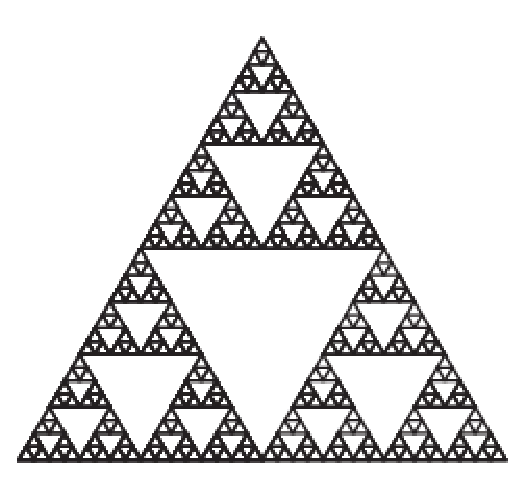
\includegraphics[width=3cm]{fractal_1}\\
\scriptsize{Figure 2. \normalfont An example of an Infinite Fractal \\(Source: \textcolor{blue}{\url{https://researchgate.net}})}}
	
A fractal is 'a rough or fragmented geometric shape that can be subdivided in parts, each of which is (at least approximately) a reduced/size copy of the whole'. The term was coined by \textit{Benoît Mandelbrot} in 1975 and was derived from the Latin fractus meaning broken or fractured.

Fractals are found in nature in the form of trees, ferns, flowers, and even river deltas. Growth Spirals follow the Fibonnaci sequence while forming fractals. A good example is that of the Romanesco Brocolli! The Human Respiratory System with its level of bronchi, bronchioles, and alveoli are proof of the omnipresence of fractals.

Two main characteristics of Fractals are:
\begin{itemize}
    \item \textbf{Self Similarity}: Every subdivision of a fractal has the same shape as the whole, i.e. self similar, which means that no matter how much one magnifies a fractal, the result would be the same.
    
    \authorIntro{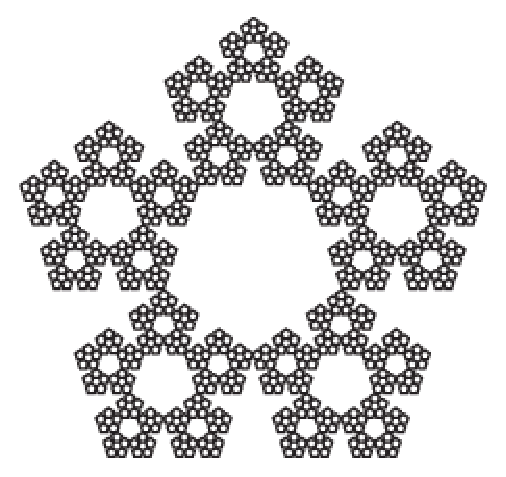
\includegraphics[width=3cm]{fractal_2}\\
    	\scriptsize{Figure 3. \normalfont A Pentagonal Fractal \\(Source: \textcolor{blue}{\url{https://researchgate.net}})}}

    \item \textbf{Non-Integer Dimensions}: Many natural phenomena don’t revolve around whole numbers and classical geometries like squares, circles, 3D cubes and spheres, e.g. \textit{Golden Ratio}, value of Pi, etc. Similarly, Fractals don’t have a dimension of a whole number, but a number between one and two dimensions. Many natural phenomena are better described using a dimension between two whole numbers.
\end{itemize}

Fractal geometry proves useful in expanding our ability to invent better devices which resonate with the surrounding nature.

The role of fractals has been crucial in development of the following areas:

\authorIntro{\includegraphics[width=3cm]{fractal_tree}\\
	\scriptsize{Figure 4. \normalfont A Fractal Tree \\(Source: \textcolor{blue}{\url{https://tomchaplin.github.io}})}}

\begin{itemize}
    \item Generation of new music, art forms
    \item Signal and Image Compression
    \item Seismology
    \item Computer Graphic designing (e.g. hills can be made through recursive algorithms of a triangle)
\end{itemize}

\subsection*{Types of fractals}

Here are some examples of Fractal patterns in nature:

\authorIntro{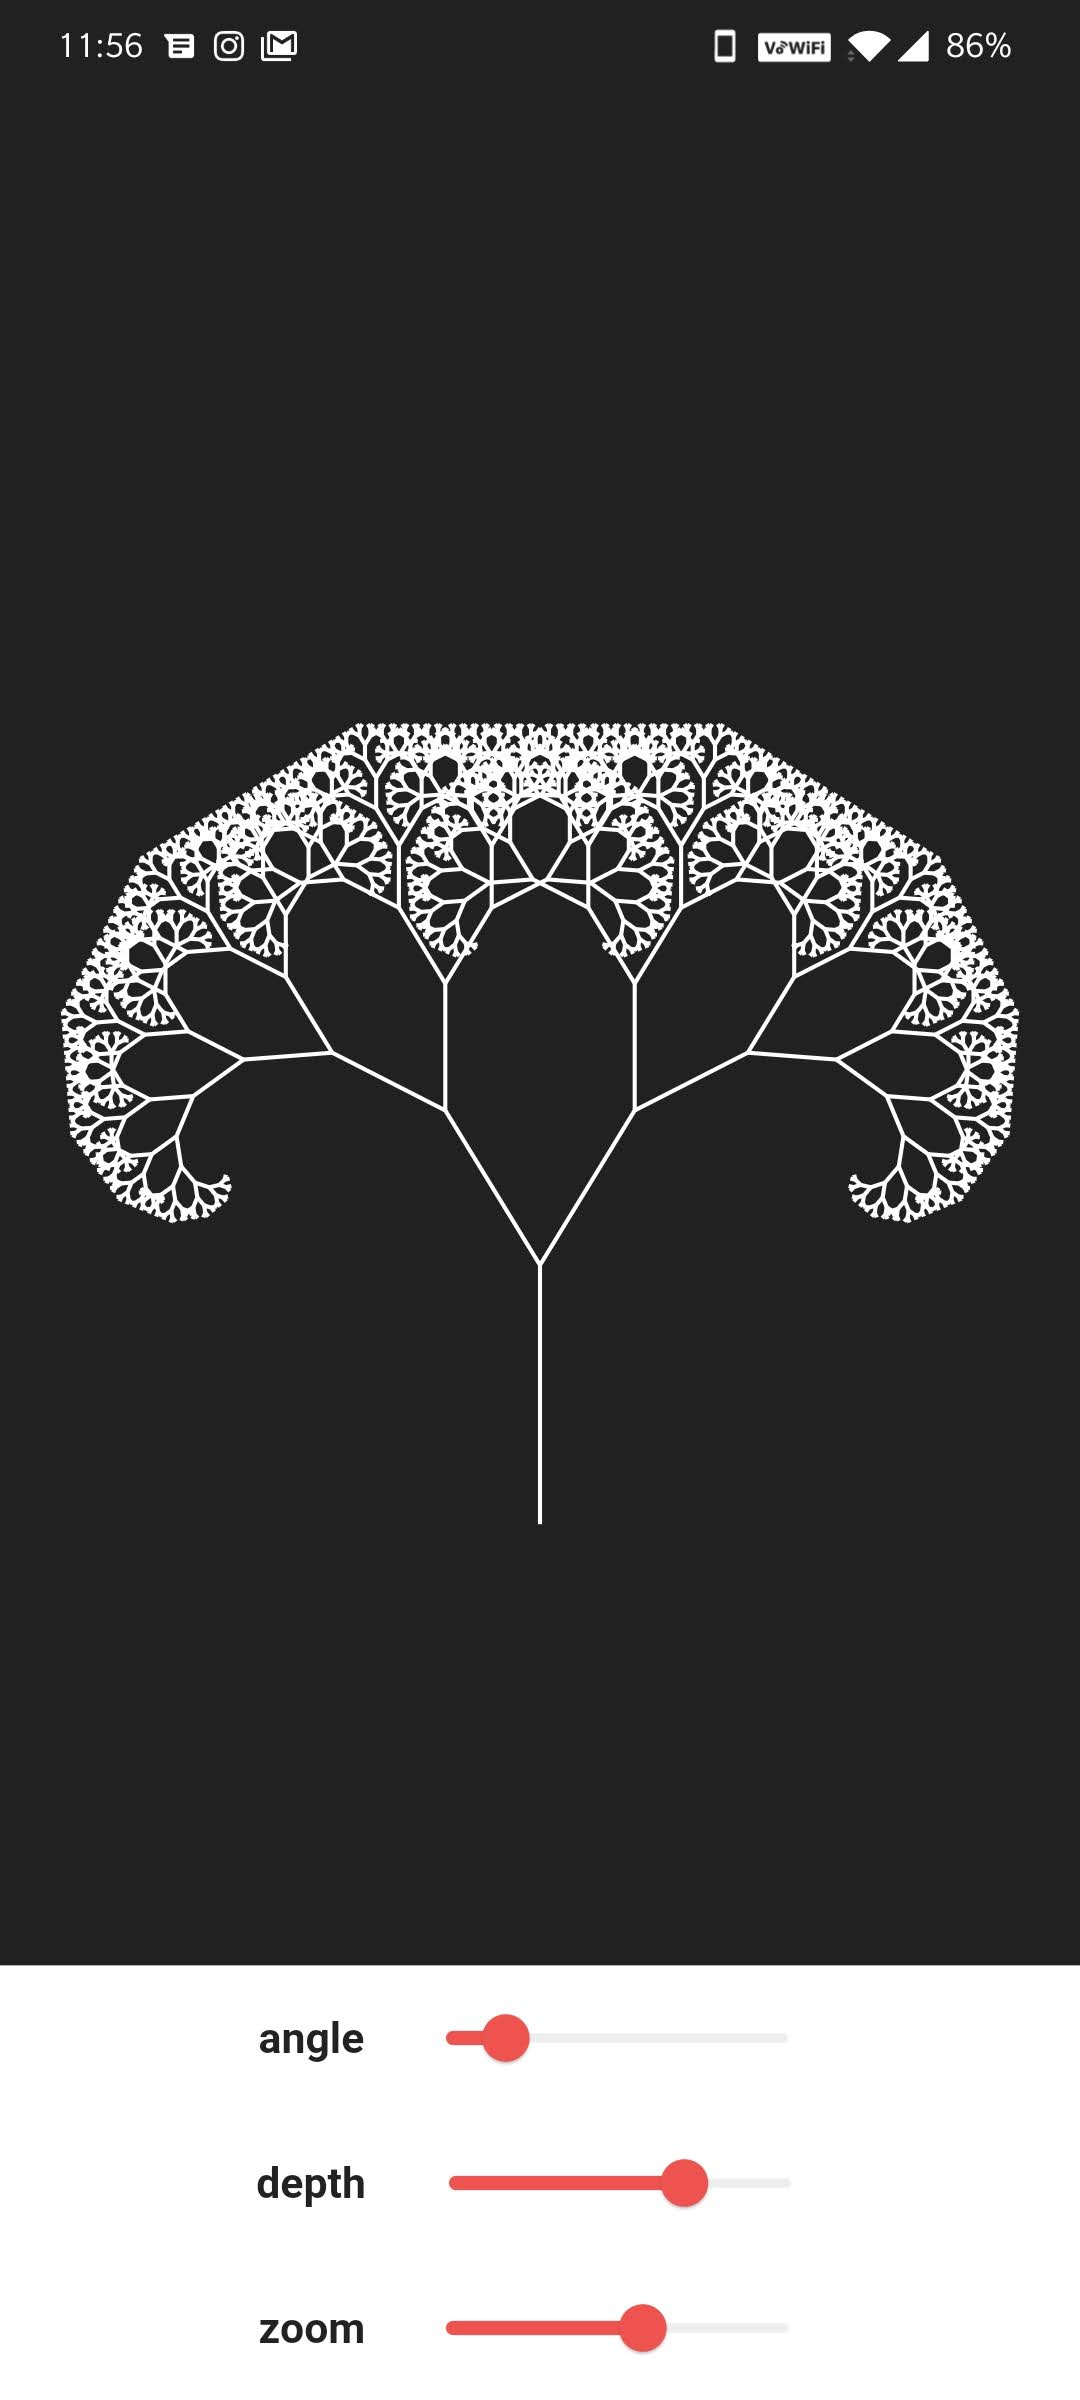
\includegraphics[width=3cm]{fractal_tree_ss_1}\\
	\scriptsize{Figure 5. \normalfont Simulating the Fractal Tree}}

\begin{enumerate}
    \item \textbf{Trees}
    \item \textbf{River Deltas}
    \item \textbf{Growth Spirals}
    \item \textbf{Flowers}
\end{enumerate}

\section*{Mathematical Foundation}
The Law of Large Numbers states that with the increase in the number of random trials, the estimated quantity becomes more accurate.\textsuperscript{[2]}

The Monte Carlo Method approximates a property of a huge distribution, by averaging that property for N of these chosen at random i.e. through drawing samples. Drawing a sample may involve the calculation of the probability of a random event or a computational simulation i.e. Monte Carlo Simulation.\textsuperscript{[4]}

Monte Carlo Methods can be expressed in \textit{mathematical terms} as follows:

Consider a multi-dimensional random variable, \textbf{X}, with its Probability Density Function (PDF) as \textbf{f\textsubscript{X}(x)}. Then, the expected value of the function \textbf{g(X)}\textsuperscript{[3]} is:

$$E(g(X)) = \sum_{x\varepsilon X} g(x)f\textsubscript{X}(x);\ if\ X\ is\ discrete$$
$$E(g(X)) = \int_{x\varepsilon X} g(x)f\textsubscript{X}(x);\ if\ X\ is\ continuous$$

Taking an N-sample of X’s, and computing the mean of \textbf{g(x)} over the sample, the Monte Carlo Approximation equals:

$$ \overline{g}\textsubscript{n}(x) = \frac{1}{n} \sum_{i=1}^{n}g(x\textsubscript{i}) $$

\section*{Algorithmic/Computer Implementation}
Let's consider an example of \textbf{trees}.


\setlength{\leftskip}{0cm}
\section{Fractal Trees}

Conventional Statistics involve characterizing surfaces. This multiple scalar nature can be depicted through fractal geometry.\textsuperscript{[5]}

To have an even clearer view of the above, we have prepared a simulation. Attached are some screenshots of the same.

In the given simulation, notice the sliders at the bottom. These represent the angle between branches, the depth of the tree, and the zoom level respectively. Even a slight change in the angle or the depth can produce an entirely different result.

Basically, the simulation of a Fractal Tree is a recursive function. It has 2 parameters:
\begin{itemize}
    \item \textbf{angle}
    \item \textbf{length}
\end{itemize}

The angle determines the angle of inclination between the current branch and its parent branch. The depth determines the depth of the tree (number of levels).

The length of the initial branch is directly proportional to the depth of the tree. After each level, the length of the branch reduces by 30\%. Thus, the bigger the depth, the denser the tree.

Here are some more screenshots:

\pagebreak

\begin{figure}[ht]
\hskip 3.27cm
\fbox{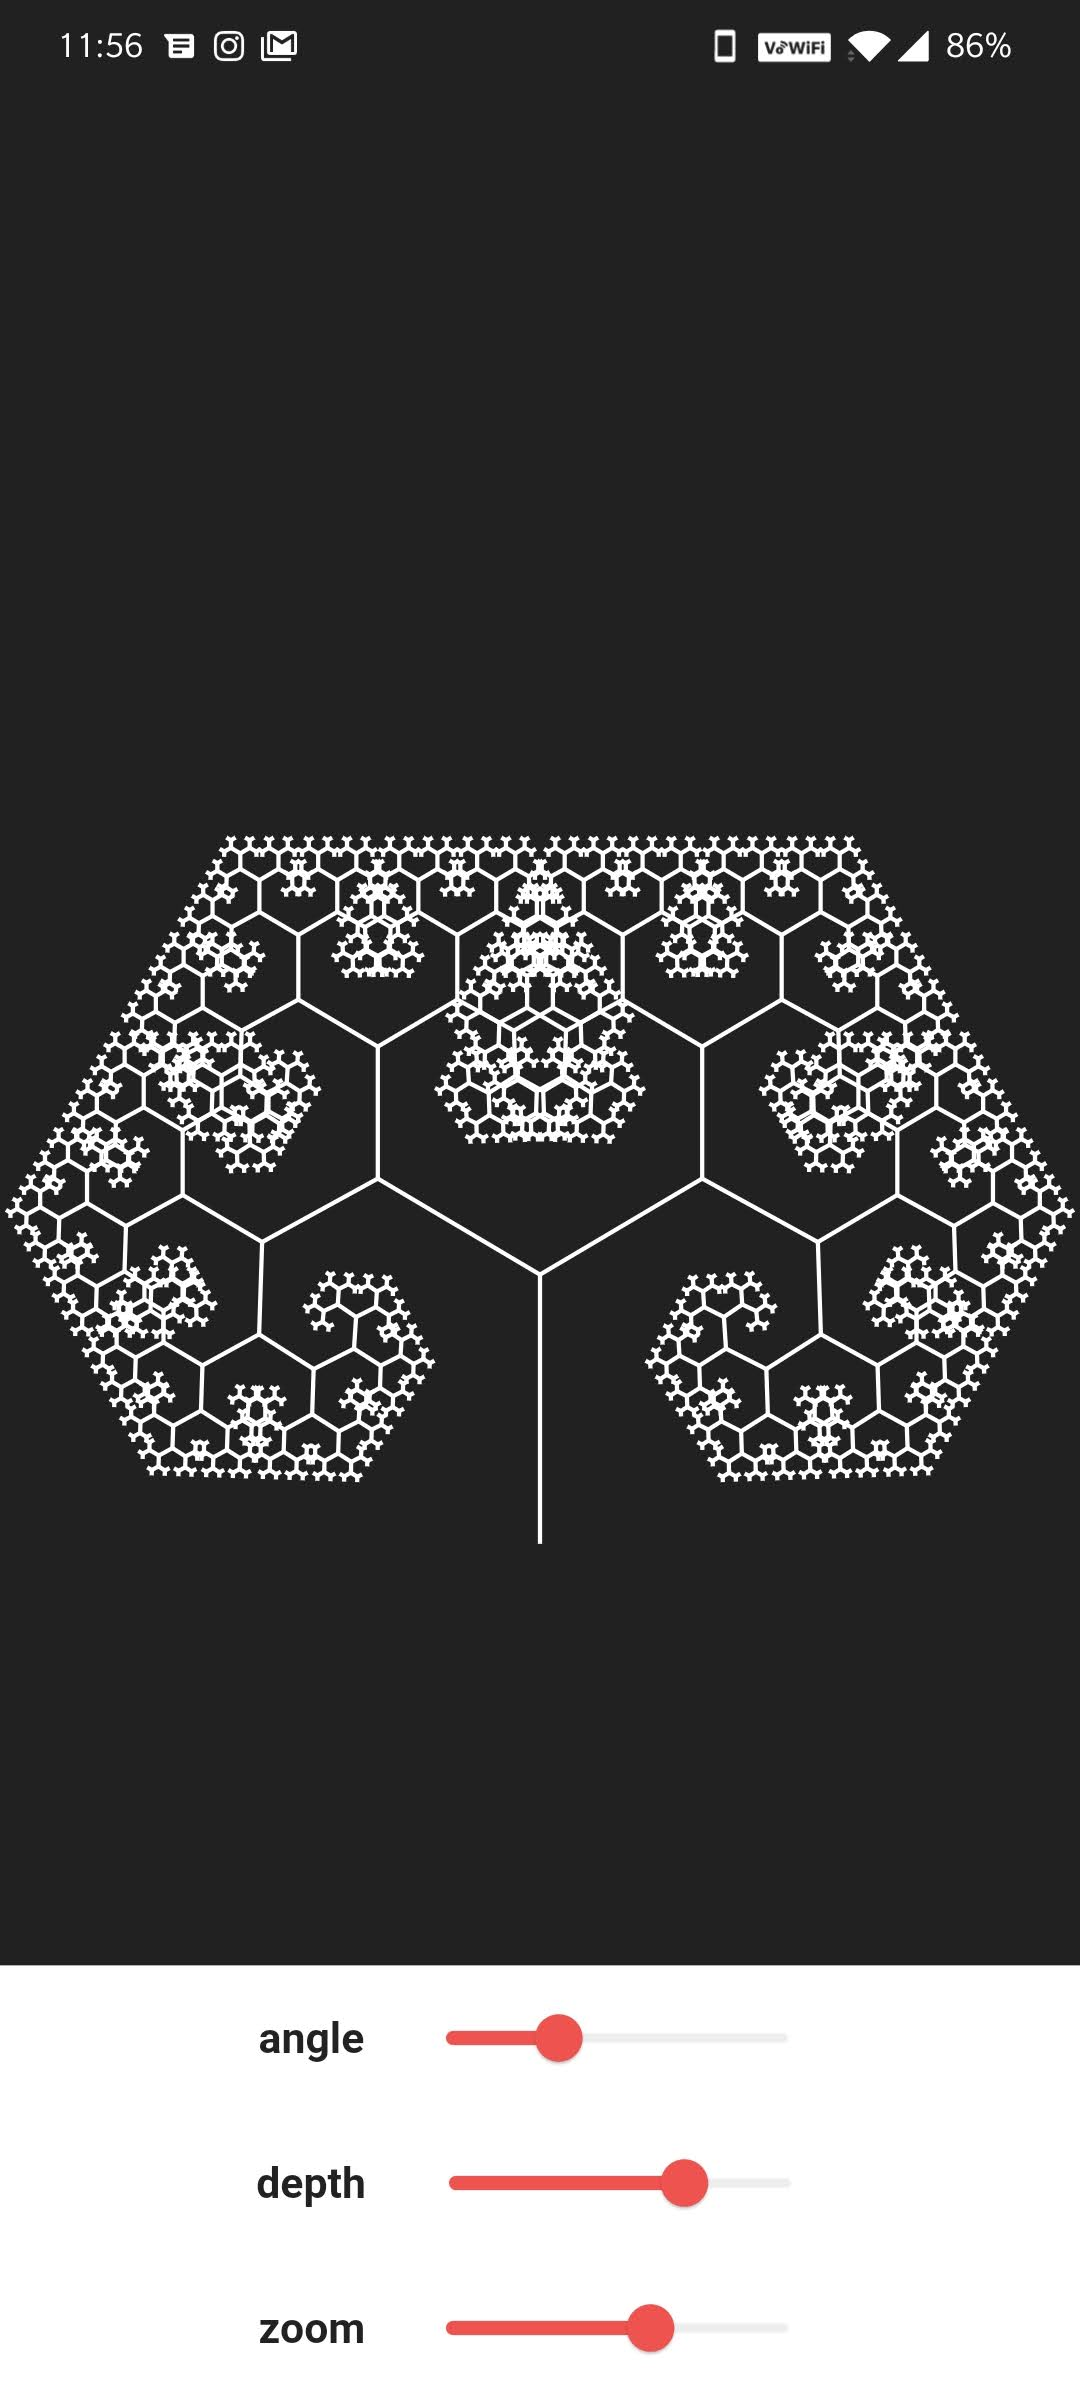
\includegraphics[width=3.3cm]{fractal_tree_ss_2}}
\fbox{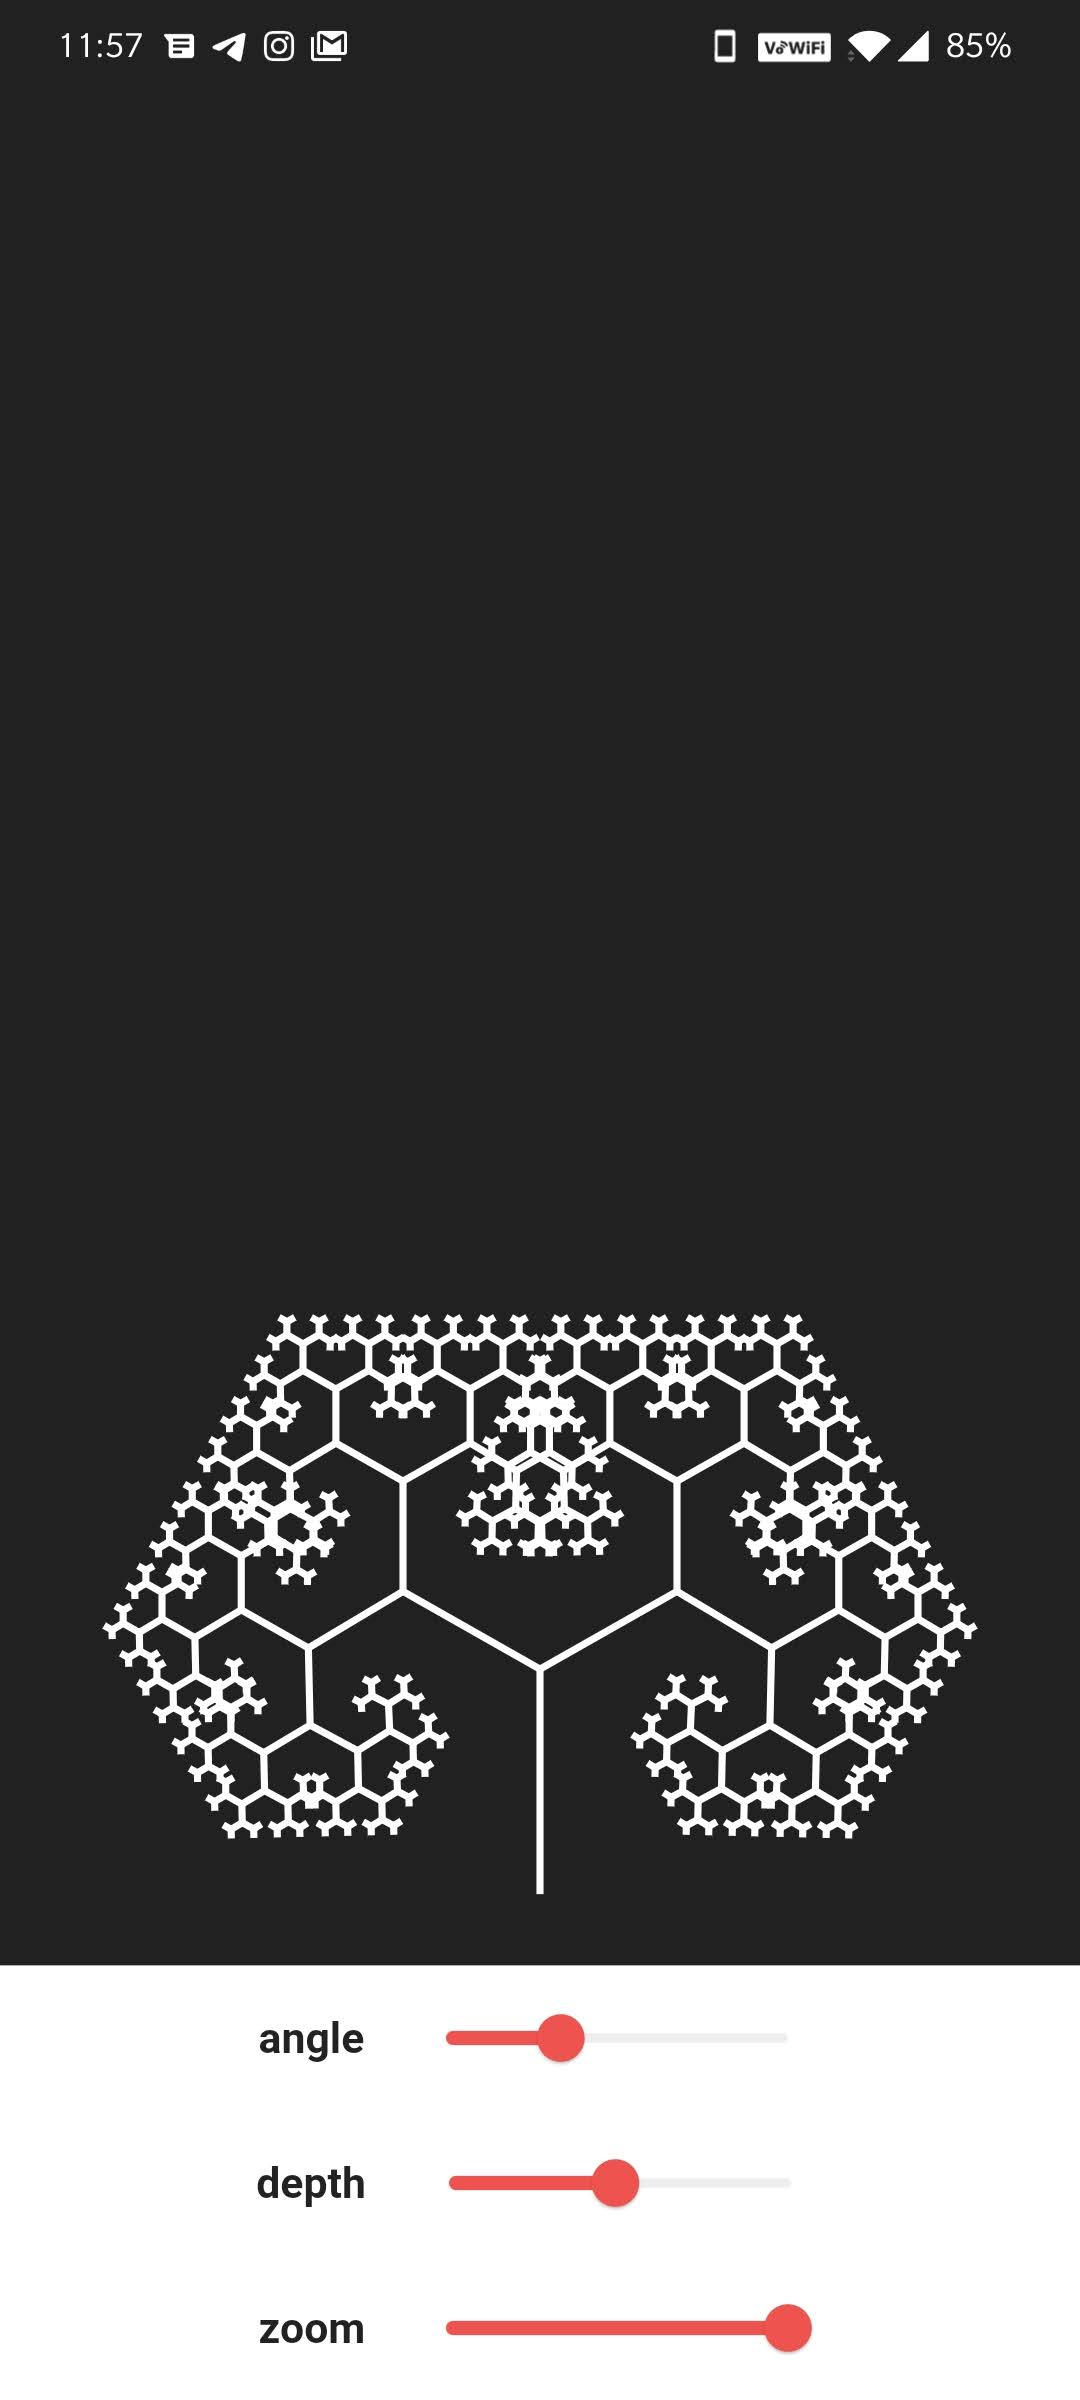
\includegraphics[width=3.3cm]{fractal_tree_ss_3}}

\vspace{10pt}
\hspace{70pt}\scriptsize{\textbf{Figure 6}. \normalfont Simulating the Fractal Tree with different rotation angles}
\end{figure}

\setlength{\leftskip}{-0cm}
Now, let's try making the tree as dense as possible.\\

\begin{figure}[h!]
    \hskip 3.27cm
    \fbox{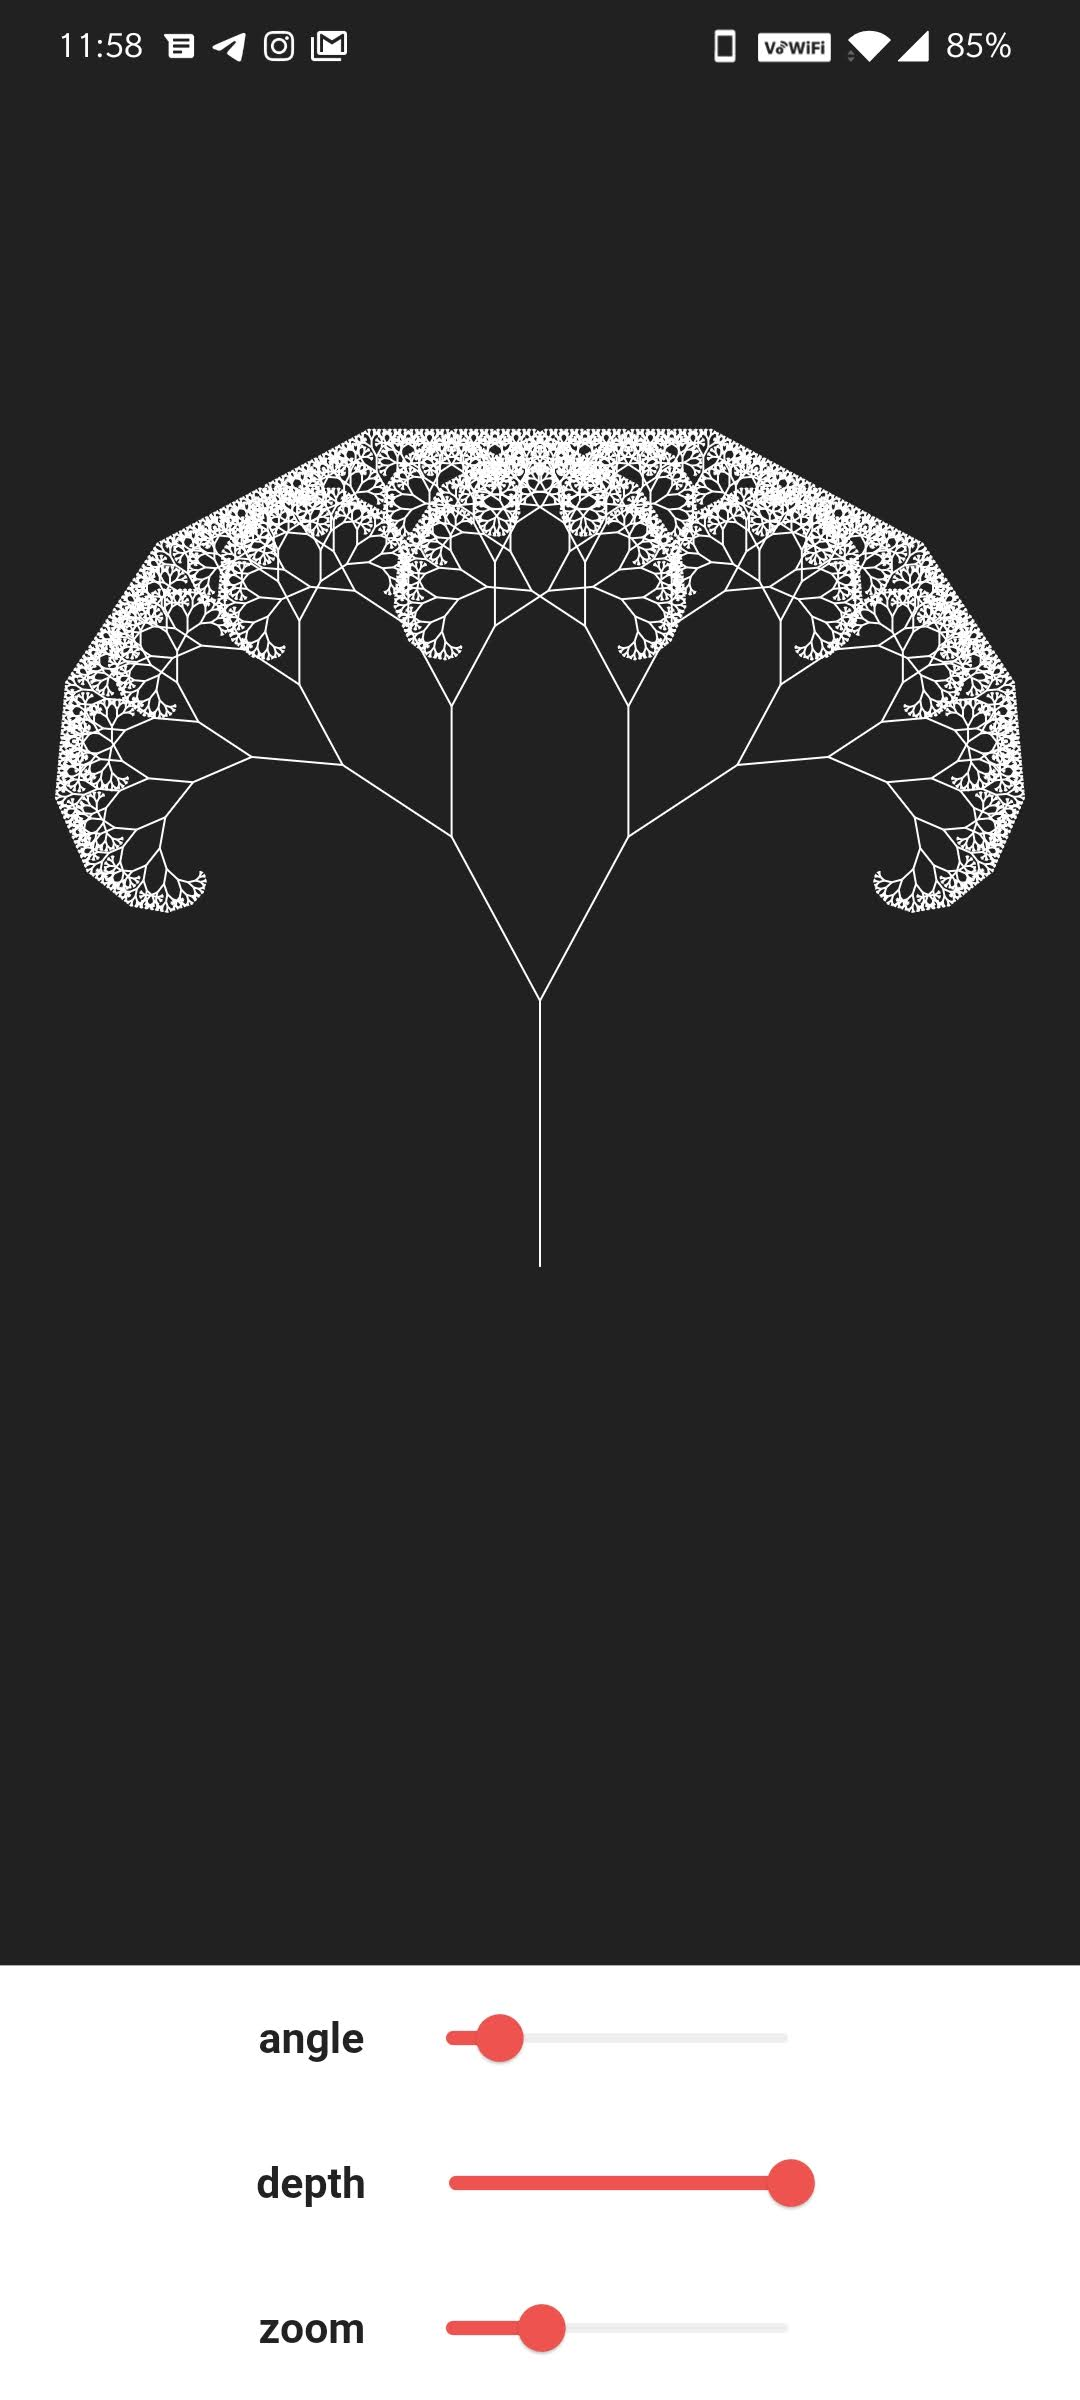
\includegraphics[width=3.3cm]{fractal_tree_ss_4}}
    \fbox{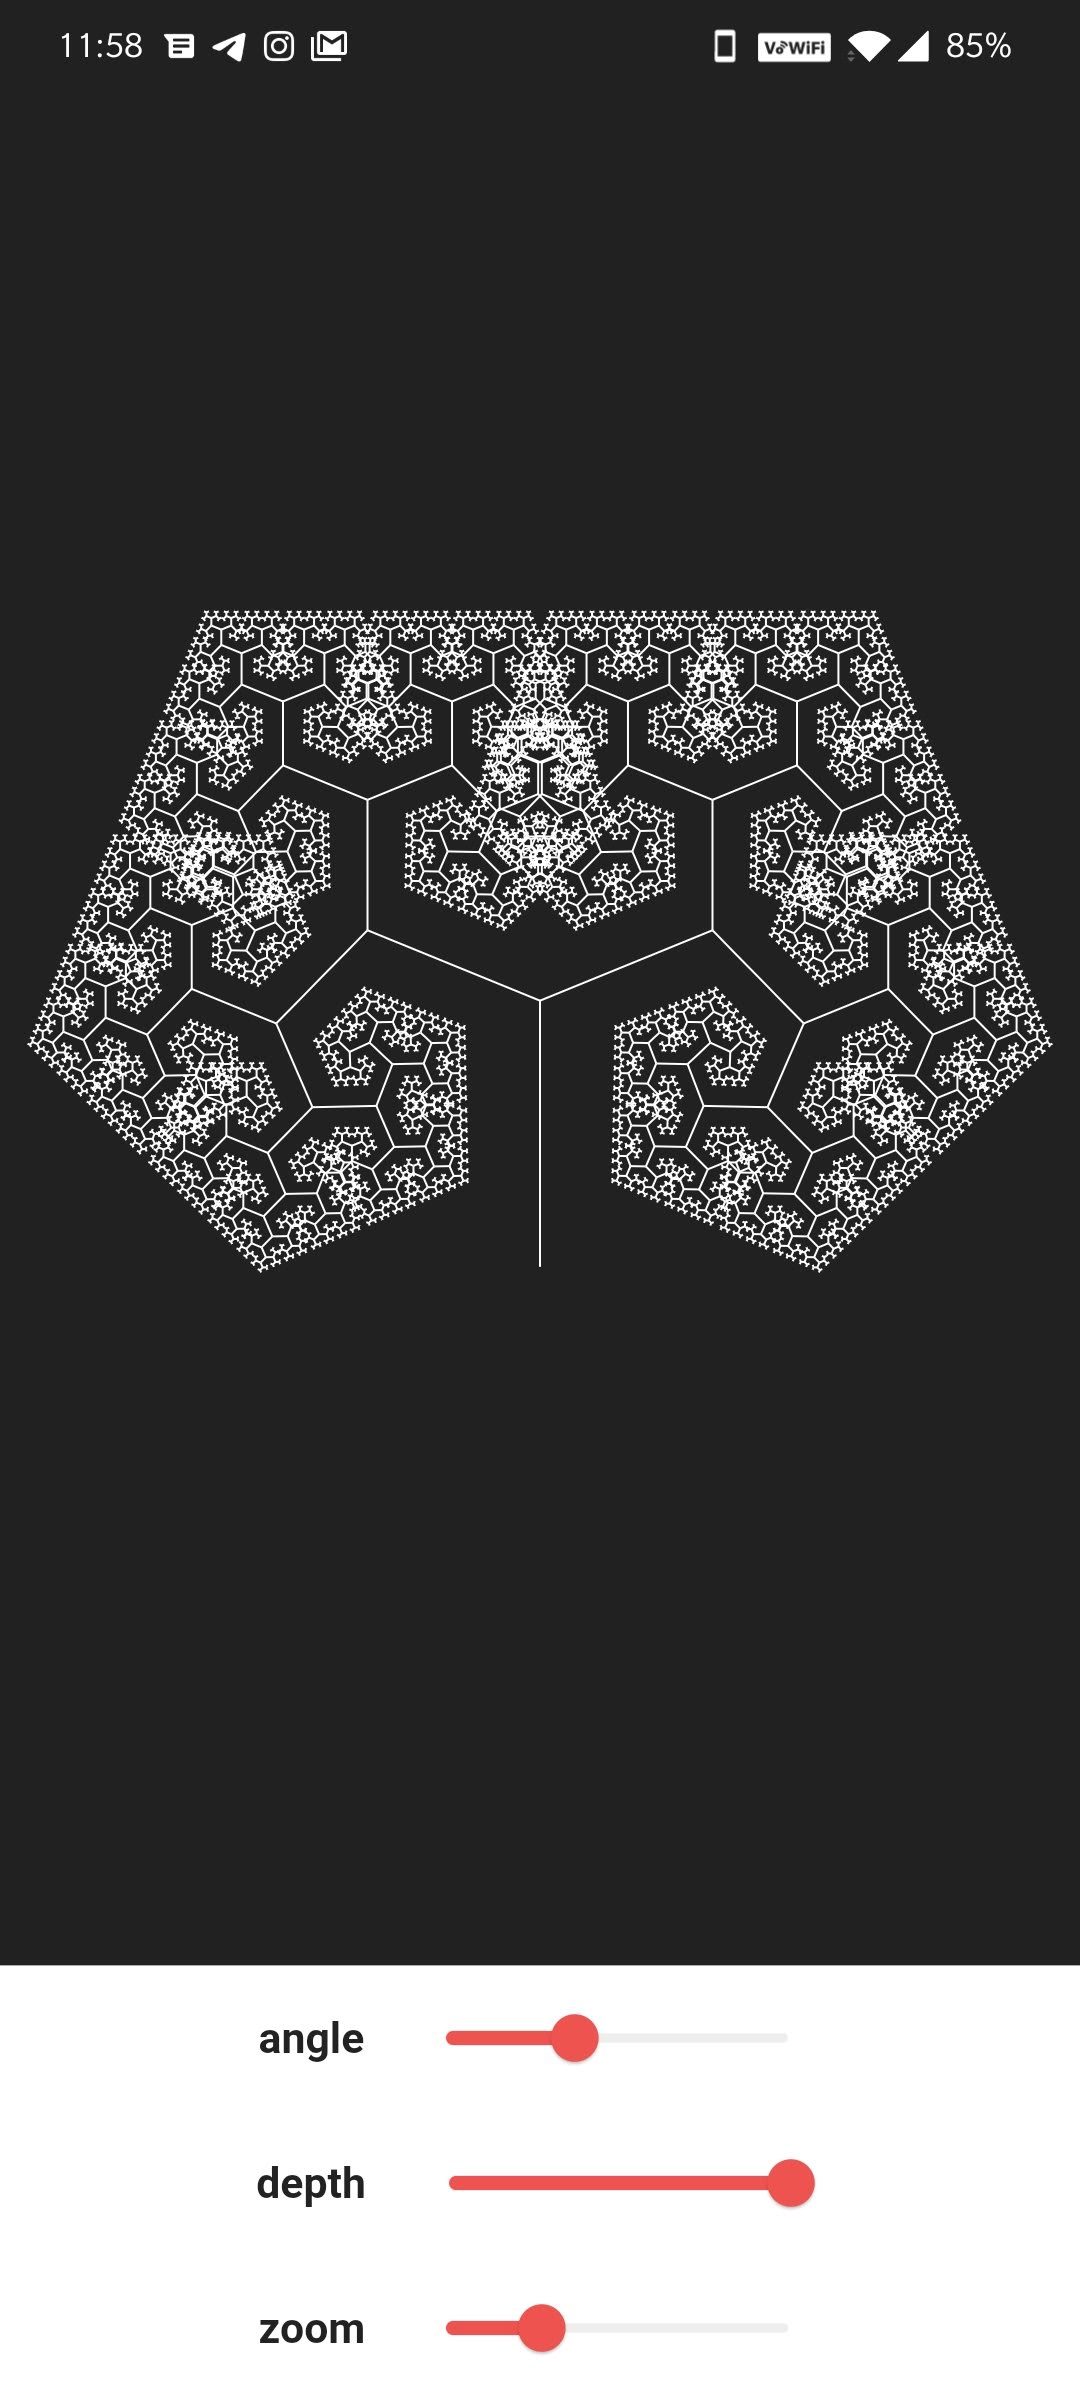
\includegraphics[width=3.3cm]{fractal_tree_ss_5}}
    
    \vspace{10pt}
    \hspace{90pt}\scriptsize{\textbf{Figure 7}. \normalfont Simulating the Fractal Tree by increasing depth}
\end{figure}

\pagebreak

The tree is much denser, and a lot taller now. Changing the angle makes the density difference look\leftHighlight{\textcolor{blue}{\url{https://bit.ly/fractals_simulation}}} even more profound. For reference, the video is hosted \textcolor{blue}{\href{https://bit.ly/fractals_simulation}{here}}.

\section{Estimation of Pi}

The plan is to simulate random \textbf{(x, y)} points on a 2-D plane with the domain as a square of side \textbf{2R} units. Consider a circle inside the same domain with the same diameter and inscribed into the square. Basically,

$$\frac{area\ of\ the\ circle}{area\ of\ the\ square}\ =\ \frac{number\ of\ points\ inside\ the\ circle}{total\ number\ of\ points\ generated}\ =\ \frac{\Pi r\textsuperscript{2}}{4r2}\ =\ \frac{\Pi}{4}\ =\ k$$

that is,

\authorIntro{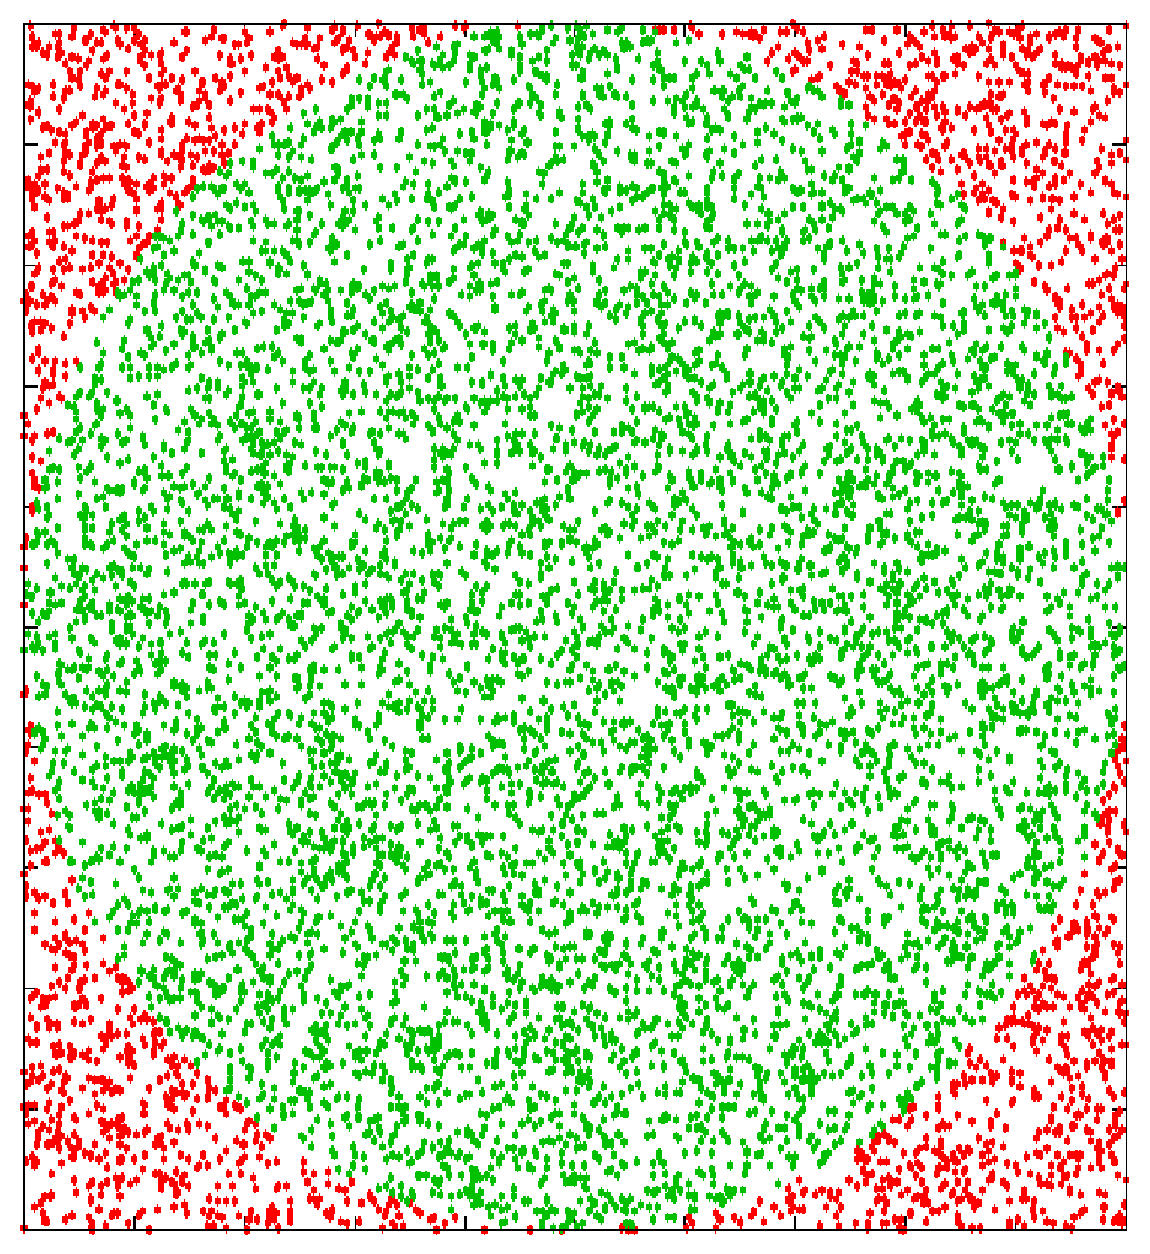
\includegraphics[width=3.5cm, height=3.5cm]{pi}\\
	\scriptsize{Figure 8. \normalfont Distribution of randomly plotted points between -R and R\\
	(Source: \\
	\textcolor{blue}{\url{www.physics.smu.edu}})}}

$$\Pi\ =\ 4\ *\ k$$

The points are generated in the \textbf{Dart} language using the \textit{dart:math} library, i.e.

$$x\ =\ rand(-R,\ R)$$
$$y\ =\ rand(-R,\ R)$$
$$where\ \textbf{rand(a,\ b)}\ generates\ random\ points\ between\ a\ and\ b$$

This is assuming that the centres of both, the square and the circle, lie at the \textbf{origin}.

Now that random points are generated, we start plotting them. If the generated point lies within the circle, we mark it with \textit{green}, else with \textit{red}. The value given by \textbf{4 * k} then evaluates to:

$$\Pi\ =\ 4\ *\ k\ =\ 4\ *\ \frac{number\ of\ green\ dots}{total\ number\ of\ dots\ (green\ +\ red)}$$

The best thing is that we don’t need to consider graphics for simulation. We only need to output random \textbf{(x, y)} pairs and then do the following:

\begin{itemize}
    \item if the point lies inside the circle - increment number of points inside the circle
    \item increment the total number of points irrespective of where the point lies
    \item calculate the above result, i.e. \textbf{4 * k}
\end{itemize}

To have a clearer view of the above, we have prepared a simulation. Here are some screenshots of the same:

\pagebreak

\begin{figure}
	\hskip 0.7cm
    \vspace{20pt}
    \fbox{\includegraphics[width=3cm]{pi_ss_1}}
    \fbox{\includegraphics[width=3cm]{pi_ss_2}}
    \fbox{\includegraphics[width=3cm]{pi_ss_3}}
    
    \vspace{-10pt}
    \hspace{30pt}\scriptsize{\textbf{Figure 9}. \normalfont Simulating the Approximation of Pi, density increasing with time}\\
\end{figure}

In the above, it is clearly evident that as the number of points increases, the approximate value of Pi approaches the real value. This is in complete agreement with the hypotheses above, and hence, proves that Monte Carlo simulations are good approximations when one can’t calculate the exact value.

\rightHighlight{\textcolor{blue}{\url{https://bit.ly/pi_approximation}}}

The complete simulation video is available \textcolor{blue}{\href{https://bit.ly/pi_approximation}{here}}.

\section{Conclusion}
In this paper, Monte Carlo simulations have been used to show two test cases:
\begin{itemize}
\item simulating Fractal Trees, and
\item estimating the value of Pi
\end{itemize}

This method has been shown to be valid and effective, through testing at various parameters.

Moreover, the simulations have proved to deliver satisfactory and expected results, whilst clearly demonstrating the feasibility of the Monte Carlo Method.\\\\\\\\\\\\\\\\

\setlength{\leftskip}{-4.2cm}
\begin{thebibliography}{99}

\vspace{5pt}
\setlength{\leftskip}{-3.8cm}
\bibitem{latexcompanion}
“A Gentle Introduction to Monte Carlo Sampling for Probability”\\ \textcolor{blue}{\url{https://machinelearningmastery.com/monte-carlo-sampling-for-probability/}}\\
{[Accessed: 7-April-2020]}\\

\bibitem{latexcompanion}
"Monte Carlo Simulations”\\ \textcolor{blue}{\url{https://www.palisade.com/risk/monte_carlo_simulation.asp}}\\
{[Accessed: 10-April-2020]}\\

\bibitem{latexcompanion}
"Mathematical Foundations of Monte Carlo Methods”\\ \textcolor{blue}{\url{https://www.scratchapixel.com/lessons/mathematics-physics-for-computer-graphics/monte-carlo-methods-mathematical-foundations/pdf-and-cdf}}\\
{[Accessed: 12-April-2020]}\\

\bibitem{latexcompanion}
"Monte Carlo Methods and Importance Sampling”\\ \textcolor{blue}{\url{http://ib.berkeley.edu/labs/slatkin/eriq/classes/guest\_lect/mc\_lecture\_notes.pdf }}\\
{[Accessed: 2-May-2020]}\\

\bibitem{latexcompanion}
Zou, Mingqing, et al. "A Monte Carlo method for simulating fractal surfaces." \textit{Physica A: Statistical Mechanics and its Applications} 386.1 (2007): 176-186.\\

\bibitem{latexcompanion}
Lin, Yi-Cheng, and Kamal Sarabandi. "A Monte Carlo coherent scattering model for forest canopies using fractal-generated trees." \textit{IEEE Transactions on Geoscience and Remote Sensing} 37.1 (1999): 440-451.\\

\bibitem{latexcompanion}
"Classification of Fractals”\\ \textcolor{blue}{\url{https://www.cs.mcgill.ca/~rwest/wikispeedia/wpcd/wp/f/Fractal.htm}}\\
{[Accessed: 28-May-2020]}\\

\bibitem{latexcompanion}
"General Introduction to Fractal Geometry”\\ \textcolor{blue}{\url{http://www.fractal.org/Bewustzijns-Besturings-Model/Fractals-Useful-Beauty.htm}}\\
{[Accessed: 31-May-2020]}\\

\bibitem{latexcompanion}
"Source of Fractals”\\ \textcolor{blue}{\url{http://www.fractal.org/Bewustzijns-Besturings-Model/Source-of-Fractals.htm}}\\
{[Accessed: 6-June-2020]}\\

\bibitem{latexcompanion}
Pippa, Natassa, et al. “On the Ubiquitous Presence of Fractals and Fractal Concepts in Pharmaceutical Sciences: A Review.” \textit{International Journal of Pharmaceutics}, Elsevier, 8 Sept. 2013,\\
\textcolor{blue}{\url{www.sciencedirect.com/science/article/pii/S0378517313008211}}

\end{thebibliography}

\pagebreak

\setlength{\leftskip}{0cm}
\section*{Annexure}

\setcounter{section}{0}
\section{Pi Approximation}

\begin{minted}{cpp}
import 'package:flutter/material.dart';
import 'package:flutter/services.dart';

import 'dart:math' as math;

main() {
  runApp(
    MaterialApp(
      debugShowCheckedModeBanner: false,
      home: MyApp(),
    ),
  );
}

class MyApp extends StatefulWidget {
  const MyApp({Key key}) : super(key: key);

  @override
  _MyAppState createState() => _MyAppState();
}

double pi = 0;

class _MyAppState extends State<MyApp> {
  @override
  Widget build(BuildContext context) {
    SystemChrome.setSystemUIOverlayStyle(
      SystemUiOverlayStyle(
        statusBarColor: Colors.grey[900],
        statusBarIconBrightness: Brightness.light,
        systemNavigationBarColor: Colors.white,
        systemNavigationBarIconBrightness: Brightness.dark,
      ),
    );

    SystemChrome.setPreferredOrientations([
      DeviceOrientation.portraitUp,
    ]);

    WidgetsBinding.instance
        .addPostFrameCallback((timeStamp) => setState(() {}));

    return Scaffold(
      backgroundColor: Colors.grey[900],
      bottomNavigationBar: BottomAppBar(
        elevation: 0,
        color: Colors.white,
        child: Padding(
          padding: EdgeInsets.symmetric(vertical: 30),
          child: Column(
            mainAxisSize: MainAxisSize.min,
            crossAxisAlignment: CrossAxisAlignment.center,
            children: <Widget>[
              Text(
                "Pi Value (approx)",
                style: Theme.of(context).textTheme.headline4.copyWith(
                      color: Colors.black,
                    ),
              ),
              SizedBox(height: 10),
              Text(
                "${pi.toStringAsFixed(12)}",
                style: Theme.of(context).textTheme.headline5,
              ),
            ],
          ),
        ),
      ),
      body: CustomPaint(
        painter: SimulationPainter(),
        child: Container(),
      ),
    );
  }
}

final coordinates = List<List<double>>();
double insideCircle = 0, total = 0;

class SimulationPainter extends CustomPainter {
  final randomGenerator = math.Random();
  double x, y;

  @override
  void paint(Canvas canvas, Size size) {
    final radius = size.width * 9 / 20;

    final paint = Paint()
      ..style = PaintingStyle.stroke
      ..strokeWidth = 2
      ..color = Colors.white;

    canvas.translate(size.width / 2, size.height / 2);

    canvas.drawCircle(Offset(0, 0), radius, paint);
    canvas.drawRect(
      Rect.fromCenter(
        center: Offset(0, 0),
        height: radius * 2,
        width: radius * 2,
      ),
      paint,
    );

    paint.style = PaintingStyle.fill;
    for (int i = 0; i < 30; i++) {
      x = -radius + randomGenerator.nextDouble() * radius * 2;
      y = -radius + randomGenerator.nextDouble() * radius * 2;

      coordinates.add([x, y]);

      ++total;
      if (x * x + y * y <= radius * radius) ++insideCircle;
    }

    coordinates.forEach((element) {
      x = element[0];
      y = element[1];

      paint.color = (x * x + y * y > radius * radius)
          ? Colors.redAccent
          : Colors.greenAccent;

      canvas.drawCircle(Offset(x, y), 0.3, paint);

      pi = insideCircle / total * 4;
    });
  }

  @override
  bool shouldRepaint(SimulationPainter oldDelegate) => true;

  @override
  bool shouldRebuildSemantics(SimulationPainter oldDelegate) => false;
}
\end{minted}

\section{Fractal Trees}

\begin{minted}{cpp}
import 'package:flutter/material.dart';
import 'package:flutter/services.dart';

import 'dart:math';

main() {
  runApp(
    MaterialApp(
      debugShowCheckedModeBanner: false,
      home: MyApp(),
    ),
  );
}

class MyApp extends StatelessWidget {
  const MyApp({Key key}) : super(key: key);

  @override
  Widget build(BuildContext context) {
    SystemChrome.setSystemUIOverlayStyle(
      SystemUiOverlayStyle(
        systemNavigationBarColor: Colors.white,
        statusBarColor: Colors.grey[900],
        statusBarIconBrightness: Brightness.light,
        systemNavigationBarIconBrightness: Brightness.dark,
      ),
    );

    SystemChrome.setPreferredOrientations([
      DeviceOrientation.portraitUp,
    ]);

    return SafeArea(
      child: AppBody(),
    );
  }
}

class AppBody extends StatefulWidget {
  AppBody({Key key}) : super(key: key);

  @override
  _AppBodyState createState() => _AppBodyState();
}

class _AppBodyState extends State<AppBody> {
  double angle = pi / 4, height = 10, scale = 0.5;
  Size size;

  @override
  Widget build(BuildContext context) {
    size = MediaQuery.of(context).size;

    return Scaffold(
      backgroundColor: Colors.grey[900],
      body: Transform.scale(
        scale: scale,
        child: CustomPaint(
          painter: FractalPainter(height, angle),
          child: Container(),
        ),
      ),
      bottomNavigationBar: BottomAppBar(
        elevation: 0,
        color: Colors.white,
        child: Column(
          mainAxisAlignment: MainAxisAlignment.center,
          mainAxisSize: MainAxisSize.min,
          children: <Widget>[
            customSlider(),
            customSlider(isHeight: true),
            customSlider(isScale: true),
          ],
        ),
      ),
    );
  }

  Widget customSlider({bool isHeight = false, bool isScale = false}) {
    return Row(
      mainAxisSize: MainAxisSize.max,
      mainAxisAlignment: MainAxisAlignment.center,
      children: <Widget>[
        Padding(
          padding: EdgeInsets.symmetric(horizontal: 10, vertical: 20),
          child: Icon(
            isHeight
                ? Icons.linear_scale
                : isScale ? Icons.zoom_in : Icons.rotate_90_degrees_ccw,
          ),
        ),
        Slider(
          min: 0,
          max: isHeight ? 20 : isScale ? 1 : pi,
          activeColor: Colors.red[400],
          inactiveColor: Colors.grey[200],
          value: isHeight ? height : isScale ? scale : angle,
          onChanged: (newValue) => setState(
            () => isHeight
                ? height = newValue
                : isScale ? scale = newValue : angle = newValue,
          ),
        ),
      ],
    );
  }
}

int counter = 0;

class FractalPainter extends CustomPainter {
  Canvas _canvas;
  Paint _paint;
  double _height, _angle;

  FractalPainter(this._height, this._angle);

  @override
  void paint(Canvas canvas, Size size) {
    _canvas = canvas;
    _paint = Paint()
      ..color = Colors.brown[800]
      ..strokeWidth = 5
      ..strokeJoin = StrokeJoin.bevel
      ..style = PaintingStyle.stroke;

    canvas.translate(size.width / 2, size.height - 30);
    drawBranch(_height * _height);
  }

  void drawBranch(double length) {
    _canvas.drawLine(Offset(0, 0), Offset(0, -length), _paint);
    _canvas.translate(0, -length);

    if (counter == length.round()) return;

    if (length > 4) {
      _canvas.save();
      _canvas.rotate(_angle);
      ++counter;
      drawBranch(length * 0.7);
      _canvas.restore();

      _canvas.save();
      _canvas.rotate(-_angle);
      ++counter;
      drawBranch(length * 0.7);
      _canvas.restore();
    }
  }

  @override
  bool shouldRepaint(FractalPainter oldDelegate) => false;

  @override
  bool shouldRebuildSemantics(FractalPainter oldDelegate) => false;
}
\end{minted}

\end{document}


